



\begin{frame}
\frametitle{Average values}

\begin{definition}
For a continuous function $f$, the \textbf{average value } of $f$ on $[a,b]$ is \[\bar{f}= f_{ave}=\dfrac{1}{b-a}\int_a^b f(x)\;dx\]
\end{definition}

%\pause
%Example:  What is the average value of $f(x)=x^2+\sin(x)$ over $[-2,2]$?

%\pause
%Example:  A hiking trail has elevation $h(x)=\frac{1}{400}x^3+4500$ (where everything is measured in feet)  What is the average height of the trail over the first 400 feet?
\end{frame}

\begin{frame}
\frametitle{What does the average value mean?}

\begin{definition}
On $[a,b]$  $\bar{f}=\dfrac{1}{b-a}\int_a^b f(x)dx$
\end{definition}

\pause

Some manipulation gives
\[
\bar{f}\cdot ({b-a}) = \int_a^b f(x)dx
\]

\pause
Geometrically, this means that the rectangle with base $b-a$ and height $\overline{f}$ has the same area as the region under the curve.


\begin{tabular}{cc}
{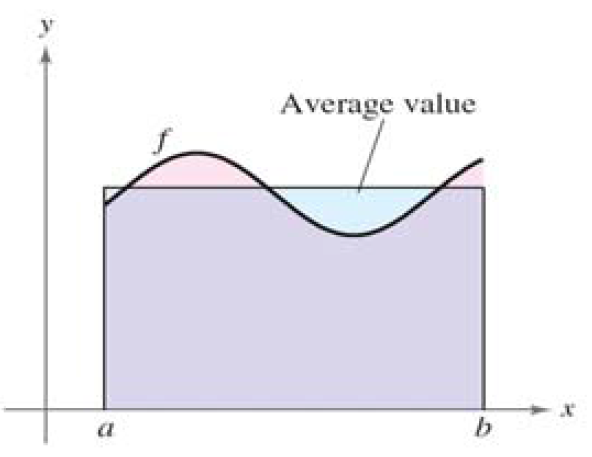
\includegraphics[width=.3\textheight]{average-value/pictures/average.pdf}}
&
\begin{tabular}[h]{l}
Pictorially, the function curve has as much\\ `area' over $\overline{f}$ as it does under.
\\
\\
%\pause
%Example:  What is the average value of $f(x)=x$ 
%\\over $[0,3]$?
\\
\\
\\
\\
\end{tabular}
\end{tabular}
\end{frame}


\begin{frame}

\frametitle{Average Value of $f(x)=\frac{1}{2}x^2$ on [0,3]}

\begin{columns}[c]
\column{.5\textwidth}
\[
f_{ave}:=\dfrac{1}{b-a} \int_a^b f(x) dx
\]
Here, $ b= $\pause $ 3 $, $ a= 0$. \pause 
 \[
 f_{\textrm{ave}}=\frac{1}{3-0}\int_0^3\frac{1}{2}x^2 dx
\]
\pause 
 \[
 =\frac{1}{3}\left(\frac{x^3}{6}\right|_0^3
\]
\pause
\[
   =\frac{1}{3}\cdot\frac{27}{6}=\frac32
 \]
 \pause 
 \column{.5\textwidth}
{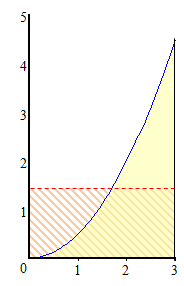
\includegraphics[width=.8\textwidth]{average-value/pictures/ex1}}
\end{columns}
\end{frame}

\begin{frame}

\frametitle{Average value of $\sin(x)$ on $[0,\pi]$.}
\[
f_{ave}:=\dfrac{1}{b-a} \int_a^b f(x) dx
\] \pause 
\begin{columns}[c]
\column{.5\textwidth}
\[
f_{av}=\frac{1}{\pi-0}\int_0^\pi\sin(x)\,dx
\]    
\pause 
\[
=\left.\frac{-\cos(x)}{\pi}\right|_0^\pi=-\frac{-1}{\pi}+\frac{1}{\pi}=\frac2\pi
\]       
\pause
 \column{.5\textwidth}
{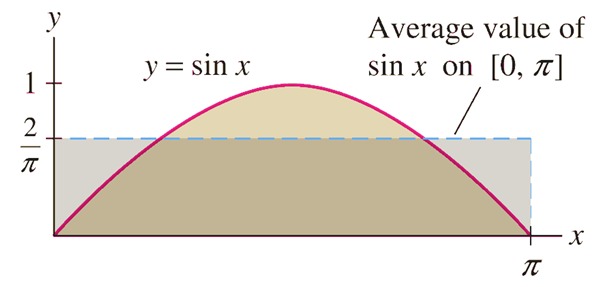
\includegraphics[width=\textwidth]{average-value/pictures/ex2}}
\end{columns}
\pause
Notice that the function takes on it's average value at the two points where the rectangle intersects the graph.

\end{frame}


\begin{frame}
\frametitle{Mean Value Theorem for integrals}

If $ f $ is not a constant function on $ [a,b] $ then  it is sometimes less than $\overline{f}$ and sometimes  greater than $\overline{f}$. (What if $ f $ IS a constant?)   Say at $x_0$ and $x_1$ we have

\[
f(x_0)<\overline{f}<f(x_1)
\]

Since $ f $ is continuous on [a,b], what does the Intermediate Value Theorem say?

\pause

\begin{theorem}[The mean value theorem for integration.]
If $f$ is continuous on $[a,b]$, then for some $c$ in $[a,b]$, $f(c)=\overline{f}:=\dfrac{1}{b-a} \int_a^b f(x) dx$
\end{theorem}

\pause

This is VERY different in the discrete (not continuous) setting. For example, the average household size in Canada according to the 2011 census survey is 2.5 people.  \pause There is no household of exactly 2.5 people.


\end{frame}


\begin{frame}

\begin{example}
{Find the value of $c$ guaranteed by the Mean Value Theorem 
for the integral of $f(x)=\frac{9}{x^3}$  over the interval [1,3].}\\

\pause 

{\bf{Solution:}}Because $f(x)$ is continuous on the interval $[1,3]$ we may apply the MVT for integrals.  
So there exists some number $c$ so that 
\[
f(c)=f_{ave}=\frac{1}{b-a}\int_a^bf(x)dx
\] 
\pause 
$\ds f_{ave}=\frac{1}{3-1}\int_1^3\frac{9}{x^3}dx$
\pause
$\ds =\frac{1}{2}\left[ -\frac{9}{2x^2}\right]_1^3$
\pause
$=\ds \frac{1}{2}\left[ -\frac12-\left(-\frac92\right)\right]$
\pause
$=2$.\\

\pause
Therefore we wish to solve $f(c)=\frac{9}{c^3}=2$  \pause which gives $c^3=\frac92$, so
\[
c=\sqrt[3]{\frac{9}{2}}
\] 




\end{example}
\end{frame}


\end{document} 